% ===================================================================================================================
% Section: Approach (25%). Needs: amsmath, booktabs, graphicx, natbib (the NeurIPS style loads it);
% \graphicspath{{figures/}}; references.bib. Numbers: epills/configs/stage2_run4.yaml, outputs/runs/stage2_run4/.
% ===================================================================================================================
\section{Method}
\label{sec:approach}

A detected pill is cropped, embedded by a hybrid CNN and ViT encoder, and compared by cosine similarity with the
patient's enrolled medicines or with a product catalogue. Decision thresholds are calibrated on validation medicines
only, and the OCR imprint reader adds complementary evidence.

The implementation adapts the team's facial expression code (\texttt{FER/}) in the project repository\footnote{\url{https://github.com/398-21/ultrasound_Model}} and the ePillID benchmark code\footnote{\url{https://github.com/usuyama/ePillID-benchmark}}. Development and report preparation are documented in Appendix~\ref{app:development}.

\subsection{Network}
\label{sec:arch}

The encoder in Figure~\ref{fig:arch} processes each $224{\times}224$ crop through a VGG16 branch~\citep{simonyan2015vgg} with CBAM channel and spatial attention~\citep{woo2018cbam} and a ViT-B/16 branch~\citep{dosovitskiy2021vit}. Local texture, colour and edge features from the CNN are combined with the ViT's global layout representation through capsule routing~\citep{sabour2017capsules}. Each branch is projected to a 256-dimensional capsule, and initially equal coupling coefficients are updated towards the branch whose features agree with the fused vector. A small transformer encoder~\citep{vaswani2017attention} then refines four 64-dimensional tokens derived from this vector, after which their mean is mapped by a linear head to the unit-length embedding $\mathbf{z}=f_\theta(x)\in\mathbb{R}^{256}$. Auxiliary heads predict shape and colour during training. The full layer configuration, pretrained checkpoints and initialisation are given in Appendix~\ref{app:configuration}, Table~\ref{tab:arch}.

\begin{figure}[!htbp]
  \centering
  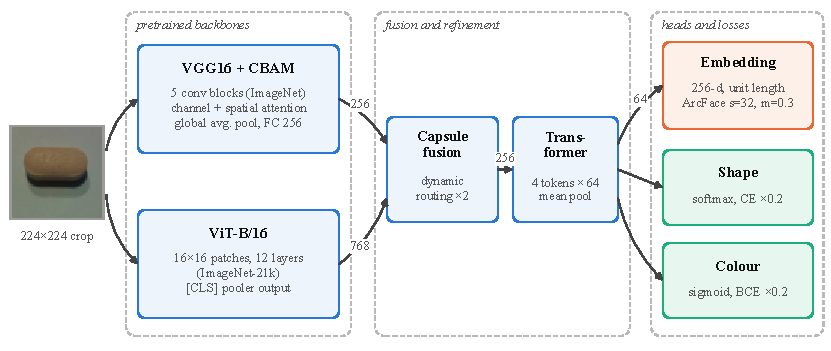
\includegraphics[width=0.98\linewidth,height=0.28\textheight,keepaspectratio]{fig02_architecture.pdf}
  \caption{The hybrid network. VGG16 with CBAM attention and ViT-B/16 see the same crop. A capsule block fuses their
    features by dynamic routing and a transformer block refines the result into a unit-length 256-d embedding trained
    with ArcFace, with auxiliary shape and colour heads. Numbers on the arrows are feature sizes.}
  \label{fig:arch}
\end{figure}



\subsection{Training}
\label{sec:training}

\paragraph{Objective.} The embedding is trained with ArcFace~\citep{deng2019arcface} over the 1,710 training
appearance groups defined in Section~\ref{sec:setup}, plus auxiliary losses:
\begin{equation}
  \mathcal{L}=-\log\frac{e^{s\cos(\theta_y+m_a)}}{e^{s\cos(\theta_y+m_a)}+\sum_{j\neq y}e^{s\cos\theta_j}}
  +\lambda_s\mathcal{L}_{\text{shape}}+\lambda_c\mathcal{L}_{\text{colour}},
  \label{eq:loss}
\end{equation}
with $s=32$, $m_a=0.3$ and $\lambda_s=\lambda_c=0.2$, where $\theta_j$ is the angle between $\mathbf{z}$ and the $j$-th
class weight, $\mathcal{L}_{\text{shape}}$ is a cross-entropy and $\mathcal{L}_{\text{colour}}$ a binary cross-entropy
(unknown labels ignored). The margin warms up over the first three epochs ($0, 0.1, 0.2$), then stays at $0.3$.

\paragraph{Optimisation.} Training follows the schedule with two phases in Table~\ref{tab:train}: the ViT and VGG blocks 1--3 are frozen during phase 1, allowing the new layers to adapt before all parameters are fine-tuned in phase 2. Each batch contains $P$ groups with $K=4$ photographs per group~\citep{hermans2017triplet}, and AdamW~\citep{loshchilov2019adamw} uses separate learning rates for pretrained backbones, new layers and the randomly initialised ArcFace class table. This separation accommodates their different initialisations, while margin warm-up introduces angular separation progressively. The combined effect of these choices is evaluated in Section~\ref{sec:ablations}.

\begin{table}[!htbp]
  \caption{Training settings of the served model (run 4). Selection: top-1 on medicines in the validation enrolment partition (best:
    phase 2, epoch 35). Seed 2026.}
  \label{tab:train}
  \centering
  \small
  \begin{tabular}{@{}lll@{}}
    \toprule
    Setting & Phase 1 & Phase 2 \\
    \midrule
    Trainable & all but ViT, VGG blocks 1--3 & all \\
    Max.\ epochs; batch ($P\times K$) & 25; $32\times4$ & 35; $16\times4$ \\
    Learning rate: backbones / new / ArcFace & $3\!\times\!10^{-5}$ / $3\!\times\!10^{-5}$ / $10^{-3}$
      & $10^{-5}$ / $10^{-5}$ / $10^{-4}$ \\
    Optimiser & AdamW, weight decay $10^{-3}$ & same \\
    Rate schedule & reduce on plateau ($\times0.5$, patience 3) & same \\
    Early stopping & patience 6, best weights restored & same \\
    \bottomrule
  \end{tabular}
\end{table}

\paragraph{Augmentation.} Colour jitter is kept small (saturation 0.05, hue 0.0125) because colour contributes to identity. Crop windows are jittered by $\times0.75$--$1.35$ with centre shifts up to 10\% to model detector error. Acquisition perturbations include brightness and contrast changes ($\pm0.3$), white balance ($\pm8\%$), downscaling to 40--160 pixels ($p=0.3$), JPEG quality 30--90 ($p=0.3$), and Gaussian noise ($\sigma=0.03$, $p=0.2$). A neighbouring pill is partly pasted into the frame with probability 0.2.

\subsection{Open-set decision rule and calibration}
\label{sec:decision}

A patient enrols each medicine $j$ from $k{=}3$ photos. Its prototype is
$\mathbf{p}_j=\sum_i f_\theta(x_{j,i})/\lVert\sum_i f_\theta(x_{j,i})\rVert$. For a query with similarities
$s_j=\mathbf{z}^\top\mathbf{p}_j$, sorted $s_{(1)}\ge s_{(2)}$,
\begin{equation}
  \hat y=\begin{cases}
    \textsc{unknown} & s_{(1)}<\tau,\\
    \textsc{retake} & s_{(1)}\ge\tau \text{ and } s_{(1)}-s_{(2)}<m,\\
    \arg\max_j s_j & \text{otherwise,}
  \end{cases}
  \label{eq:decision}
\end{equation}
where \textsc{retake} requests another photograph with the pill turned over. Calibration uses validation medicines in 1,000 simulated ten-medicine galleries, yielding $\tau=0.895$ for 95\% rejection of foreign medicines and $m=0.115$ as the largest margin with at most 10\% retakes. The crop window is selected as $1.55\times$ the detected box's long side from a sweep of 1.3--2.0, across which correct naming varies by approximately one percentage point (Figure~\ref{fig:calib}b).



\subsection{Identification with imprints and calibrated confidence}
\label{sec:identify}

For catalogue identification, a pill outside the personal gallery is ranked against 4,936 US products using each product's similarity to its closest reference as its appearance score $s$. Florence-2-large~\citep{xiao2024florence2} reads the imprint zero-shot at
four rotations (Florence-2-base for inference on a central processing unit (CPU)). Each recorded imprint token receives an inverse document frequency (IDF) weight in $[0,1]$, assigning greater weight to rare tokens such as `EC5' than to common tokens such as `93', which appears on hundreds of Teva pills. A product's imprint
score $r$ is the weight of its best token found in the reads, and the top $K{=}100$ products by look are re-ranked by
$s+\alpha r$ with $\alpha=0.05$, both chosen on validation (Figure~\ref{fig:identify}b). In the patient's gallery, only
tokens that distinguish the enrolled imprints from each other confirm or contradict a match. Catalogue confidence is estimated by logistic calibration~\citep{platt1999probabilistic} from the top candidate's appearance score, its separation from the runner-up and its imprint evidence. 

Raw cosine similarities are not probabilities: even products outside the catalogue can obtain similarities around 0.93. The fitted catalogue confidence is
\begin{equation}
  \sigma\!\left(-12.50+12.50s_1+72.13(s_1-s_2)+3.92r_1\right),
\end{equation}
where $s_1$ and $s_2$ are the appearance scores of the first two re-ranked products and $r_1$ is the first product's imprint score. This estimate concerns correctness of catalogue candidates, while gallery membership and ambiguity remain governed by Equation~\ref{eq:decision}.

\subsection{Implementation and reproducibility}
Training uses PyTorch~\citep{paszke2019pytorch} 2.11 and Hugging Face Transformers 5.19 on one NVIDIA RTX 4080 SUPER graphics processing unit (GPU) with 16\,GB memory. The deployed model is served through FastAPI on a Hugging Face ZeroGPU Space\footnote{\url{https://davidpansx-pharmascan-api.hf.space/ui/}}. Split generation, training, calibration and evaluation are separate scripts. The execution commands and output conventions are provided in Appendix~\ref{app:development}.

\subsection{Software 3.0 in coding and evaluation}
\label{sec:sw3-approach}\label{sec:sw3-experiments}
The evaluation harness was written with the coding agent from specifications in natural language, covering patient simulation, look-alike stress tests and comparisons of products from the same manufacturer, top-$k$ and confidence evaluation, figure generation, and the API's 92 tests. Testing and review identified defects including an error in the label reader that linked an extended-release sticker to the immediate-release product, which was corrected by enforcing the release form. Procedural safeguards comprised selection of settings on validation data, one evaluation of each test set, and files generated by scripts as the source of reported numerical results.
